\section{Scenario and Problem Statement}
\label{sec:scenario}
Our research is motivated by the need to enable situational understanding in coalition military operations. Militaries are increasingly using technology to help achieve this goal, deploying a variety of intelligent sensors for collecting and analyzing data. This has led to the development of the “Internet of Battlefield Things” (IoBT) concept to describe future military operations. In the IoBT, the “things” (e.g. sensors, vehicles, robots, wearable devices) will be augmented with various levels of intelligence, and will communicate with each other to coordinate their operations, as well as with their human users to facilitate sensemaking~\cite{Kott:2016, Suri:2016}.

The battlefield setting presents a number of barriers to achieving this vision. Information flow constraints are a major challenge: devices will be distributed and move around over a wide geographical area, often in regions with poor or no communications infrastructure. Communications will need to be wireless -- for example via satellite link or cellular networks -- but these methods suffer from high latency, as well as being potentially costly. The current popular model of providing devices with intelligent behaviours by transferring their data to back-end cloud services for processing will not be possible. Devices will therefore require local data processing and intelligence capabilities~\cite{Verma:2017}.

However, edge devices are also locally resource-constrained in terms of compute capability and energy consumption. A particular device may be serving many different requests from different users, and with limited local compute capacity could quickly become overloaded. If battery powered, the device will also need to minimize its energy consumption by reducing the number of computations it performs, while still remaining useful to the coalition.

In this paper, we explore a method that addresses these issues in the case of edge devices running deep neural networks (DNNs). DNNs have proven extremely effective for a variety of machine learning tasks including data classification, time-series prediction, anomaly detection, and speech/language processing~\cite{LeCun:2015, Goodfellow:2016}. The power of DNNs comes from their capacity to learn rich, hierarchical representations from data~\cite{Bengio:2013}. The term “deep” refers to the number of layers used to learn these representations. For complex data such as video, audio, or images, deeper models with more layers tend to perform better than shallower models~\cite{Szegedy:2015}. However, as the depth of the model increases, so do the computational requirements, meaning that DNNs may not be practical for deployment on computationally-limited or energy-constrained edge devices.

We propose exploiting the hierarchical nature of the learned representations in a DNN to adaptively distribute the computation over the edge devices in the coalition network. Our method builds on work by Panda et al., which showed how the energy consumption of DNN computation could be reduced by considering the output of one network layer at a time, and only computing the output of the next layer if the confidence of the output based on the current layer was low~\cite{Panda:2016}. This minimizes computational requirements by cutting out unnecessary processing by deeper layers for “easier” inputs. Our approach proposes distributing the computation of different layers between different devices on the network. Using this scheme, the processing requirements on the first device are minimised, and if further processing by deeper layers is required, another device can be called on to do this if the first device needs to reduce its computational load. This process can be chained, potentially involving as many devices as there are network layers.

\begin{figure}[ht]
\centering
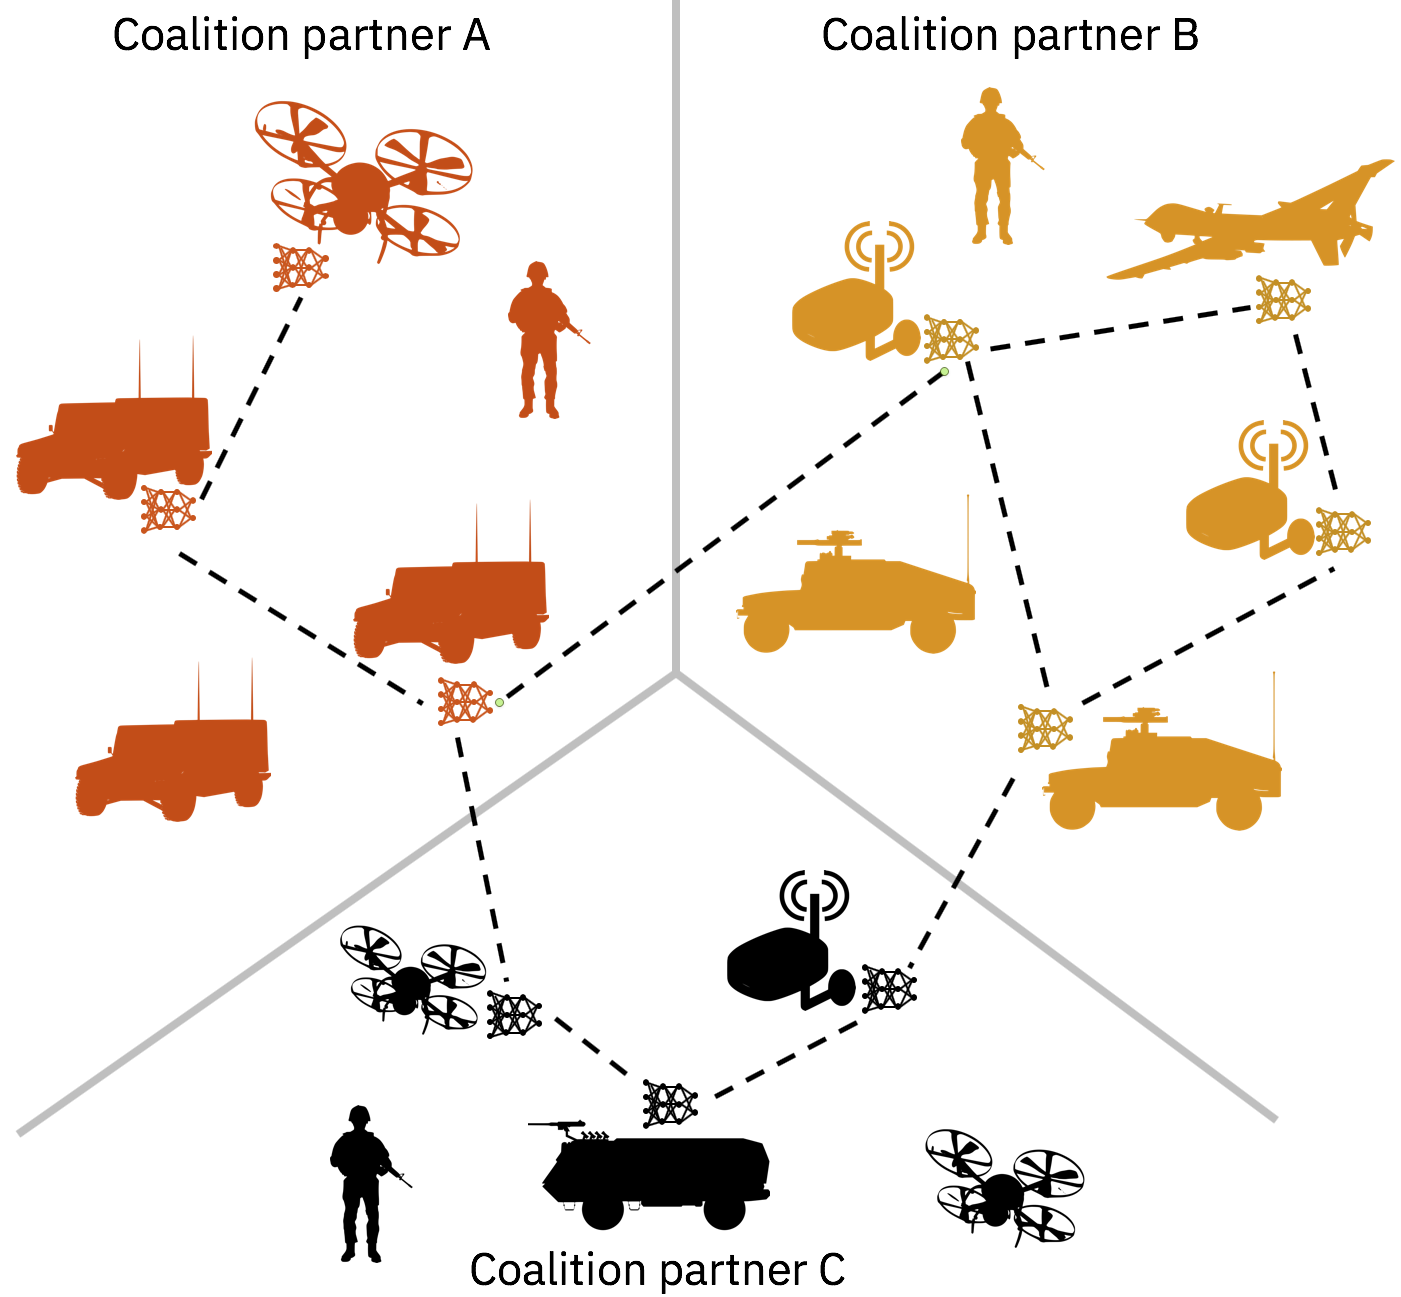
\includegraphics[width=0.49\textwidth]{fig1.png}
\caption{Conceptual illustration of the IoBT, and the proposed distribution method for DNNs. In this example, three coalition partners are collaborating. Each partner has deployed intelligent devices to the battlefield. Several of these devices have the same DNN deployed on them, and so can distribute computation between them layer by layer.}
\label{fig:coalition}
\end{figure}